\chapter{Resultados y discusión de la tesis}
En este capítulo se mostrarán los resultados obtenidos al realizar las pruebas con el sistema de seguridad para el control de acceso por reconocimiento de voz que fue diseñado e implementado anteriormente, y así poder ver si se obtuvieron los objetivos alcanzados y poder comparar las ventajas y desventajas del proyecto propuesto.
\vskip 0.5cm
Las pruebas están divididas en 2 partes, la primera consiste en obtener los umbrales de decisión para las respuestas del sistema (Identificación Correcta, Falsa Identificación y No Identificación) y la segunda parte consiste en evaluar el algoritmo de construcción del patrón de referencia definida por la Ecuación \eqref{eq:ecuacion101} para la reducción del tiempo de ejecución en la respuesta del sistema.
\vskip 0.5cm
Para la realización de las pruebas se escogió un lugar con un nivel de ruido bajo de 69 a 78 dBC. Además, se utilizaron a 11 personas del sexo masculino con edades entre 22 a 24 años, esto porque es evidente que para el algoritmo le resultará más fácil diferenciar un hombre de una mujer y un niño de un adulto debido algunos aspectos físicos en el tracto vocal que se explicó en la teoría, por ello se escogió a personas del mismo sexo con edades parecidas, así al sistema le resultará más difícil realizar el reconocimiento de voz. A continuación, definiremos algunas abreviaturas que usaremos para la realización de las pruebas:
\begin{enumerate}
\item[-]\textit{U1}: Umbral de decisión para reconocer la palabra
\item[-]\textit{U2}: Umbral de decisión para reconocer al locutor
\item[-]\textit{U}: Umbral de decisión definido por la Ecuación \eqref{eq:ecuacion105}
\item[-]\textit{IC}: Respuesta del sistema de identificación correcta
\item[-]\textit{FI}: Respuesta del sistema de falsa identificación
\item[-]\textit{NI}: Respuesta del sistema de no identificación
\item[-]\textit{A}: Respuesta de acierto en el reconocimiento
\item[-]\textit{D}: Respuesta de desacierto en el reconocimiento
\item[-]\textit{E}: Error de respuesta del sistema
\end{enumerate}
En la ejecución de las pruebas se presentarán 8 escenarios o casos distintos, que a continuación pasaremos a explicar cada una de ellos:
\begin{enumerate}
\item[•]Caso 1: Para este caso se empleó a 10 usuarios, cada uno de ellos dijo como palabra clave de acceso su nombre 40 veces (\textit{ANTONY}, \textit{CARLOS}, \textit{EDINSON}, \textit{EDWIN}, \textit{GERSON}, \textit{JORDAN}, \textit{JOSUE}, \textit{NIZAMA}, \textit{OCAS} y \textit{RENZO}). De las 40 grabaciones que se obtuvo por cada usuario 30 de ellas pasaran a la etapa de entrenamiento y las otras 10 para las pruebas, haciendo un total de 300 audios para la base de datos y 100 audios para la realización de la prueba.
\item[•]Caso 2: Para este caso se empleó a 10 usuarios, cada uno de ellos dijo como palabra clave de acceso \textit{ABRIR} 40 veces. De las 40 grabaciones que se obtuvo por cada usuario 30 de ellas pasaran a la etapa de entrenamiento y las otras 10 para las pruebas, haciendo un total de 300 audios para la base de datos y 100 audios para la realización de la prueba.
\item[•]Caso 3: Para este caso se empleó a 10 usuarios, cada uno de ellos dijo como palabra clave de acceso su nombre 30 veces (\textit{ANTONY}, \textit{CARLOS}, \textit{EDINSON}, \textit{EDWIN}, \textit{GERSON}, \textit{JORDAN}, \textit{JOSUE}, \textit{NIZAMA}, \textit{OCAS} y \textit{RENZO}), haciendo un total de 300 audios en la base de datos para la etapa de entrenamiento. Luego cada uno de los usuarios intentará acceder diciendo la palabra \textit{ABRIR} 10 veces, generando un total de 100 audios para la realización de la prueba.
\item[•]Caso 4: Para este caso se empleó a 10 usuarios, cada uno de ellos dijo como palabra clave de acceso \textit{ABRIR} 30 veces, haciendo un total 300 audios en la base de datos para la etapa de entrenamiento. Luego cada uno de los usuarios intentará acceder diciendo su nombre 10 veces (\textit{ANTONY}, \textit{CARLOS}, \textit{EDINSON}, \textit{EDWIN}, \textit{GERSON}, \textit{JORDAN}, \textit{JOSUE}, \textit{NIZAMA}, \textit{OCAS} y \textit{RENZO}), haciendo un total de 100 audios para la realización de la prueba.
\item[•]Caso 5: Para este caso se empleó a 11 usuarios, donde 10 de ellos dijeron como palabra clave de acceso sus nombres 30 veces (\textit{ANTONY}, \textit{CARLOS}, \textit{EDINSON}, \textit{EDWIN}, \textit{GERSON}, \textit{JORDAN}, \textit{JOSUE}, \textit{NIZAMA}, \textit{OCAS} y \textit{RENZO}), haciendo un total de 300 audios en la base de datos para la etapa de entrenamiento. Luego el usuario faltante (usuario no registrado) tratará de acceder con las palabras clave de acceso de los usuarios registrados, pronunciando 10 veces los nombres de cada usuario registrado, generando un total de 100 audios para la realización de la prueba.
\item[•]Caso 6: Para este caso se empleó a 11 usuarios, donde 10 de ellos dijeron como palabra clave de acceso \textit{ABRIR} 30 veces, haciendo un total de 300 audios en la base de datos para la etapa de entrenamiento. Luego el usuario faltante (usuario no registrado) tratará de acceder con la palabra clave de acceso \textit{ABRIR}, pronunciando 100 veces esta palabra, generando un total de 100 audios para la realización de la prueba.
\item[•]Caso 7: Para este caso se empleó a 11 usuarios, donde 10 de ellos dijeron como palabra clave de acceso sus nombres 30 veces (\textit{ANTONY}, \textit{CARLOS}, \textit{EDINSON}, \textit{EDWIN}, \textit{GERSON}, \textit{JORDAN}, \textit{JOSUE}, \textit{NIZAMA}, \textit{OCAS} y\textit{ RENZO}), haciendo un total de 300 audios en la base de datos para la etapa de entrenamiento. Luego el usuario faltante (usuario no registrado) tratará de acceder con la palabra \textit{ABRIR}, pronunciando 100 veces esta palabra, generando un total de 100 audios para la realización de la prueba.
\item[•]Caso 8: Para este caso se empleó a 11 usuarios, donde 10 de ellos dijeron como palabra clave de acceso \textit{ABRIR} 30 veces, haciendo un total de 300 audios en la base de datos para la etapa de entrenamiento. Luego el usuario faltante (usuario no registrado) tratará de acceder con los nombres de los usuarios registrados, pronunciando 10 veces los nombres de cada usuario registrado, generando un total de 100 audios para la realización de la prueba.
\end{enumerate}

\section{Pruebas para obtener los umbrales de decisión}
Esta parte consta de 2 etapas, la primera será en hallar $U2$ valor que nos permitirá decir si es o no el locutor ante una falsa identificación además $U1$ tendrá como valor a $U$, una vez obtenido el mejor valor para $U2$ pasaremos a la segunda etapa que consiste en hallar $U1$ valor que nos permitirá decir si es o no la palabra hablada.
\vskip 0.5cm
Los valores de $A$ y $D$ determinan el grado de acierto de nuestro algoritmo en la etapa de reconocimiento, por ejemplo para el caso 1 si se tiene que $A = 100$ y $D = 0$, esto quiere decir que el algoritmo de reconocimiento de voz obtuvo el patrón de referencia correcto (es el locutor y es la palabra) para cada audio de prueba, con esto podemos decir que el algoritmo alcanzó un 100\% de tasa de acierto en la etapa de reconocimiento.

\subsection{Prueba para obtener U2}
\par
En esta primera prueba se obtuvo que el mejor valor para $U2$ es 0.31. Esto porque, se observó que para los casos 3, 4, 5, 7 y 8 cualquier valor que tome $U2$ entre 0.20 y 0.35 el valor de $E$ es el mismo, por lo que no se tomó en cuenta a estos casos, entonces de los casos 1 y 2, ver Tablas \ref{table:tabla4.1} y \ref{table:tabla4.2}, se observó que el mejor valor para $U2$ es 0.35 dando $E = 0$ alcanzando una tasa de acierto del 100\% en la respuesta del reconocimiento de voz, ver la Figura \ref{fig:figura4.1}, sin embargo, para el caso 6 el valor de $IC$ sería 5, ver Tabla \ref{table:tabla4.6}, esto quiere decir que de las 100 veces que el intruso intento acceder en 5 de ellas el sistema le permitió el acceso, y esto es grave porque que nosotros lo que buscamos es la seguridad, por lo que $U2$ tendrá que ser menor que 0.32 y mayor que 0.30 para que el número de $FI$ no sea grande para los casos 1 y 2, por lo que se escogió a 0.31, ver la Figura \ref{fig:figura4.2}.

\begin{center}
\begin{table}[H]
\centering
\caption{\small{Resultados para obtener U2 en el caso 1.}}
\label{table:tabla4.1}
\vskip 0.2cm
\scalebox{0.7}{
\begin{tabular}{|c|c|c|c|c|c|c|c|}
\hline 
U1 & U2 & IC & FI & NI & A & D & E \\
\hline 
U & 0.20 & 50 & 50 & 0 & 100 & 0 & 50 \\
\hline 
U & 0.21 & 57 & 43 & 0 & 100 & 0 & 43 \\
\hline 
U & 0.22 & 61 & 39 & 0 & 100 & 0 & 39 \\
\hline 
U & 0.23 & 65 & 35 & 0 & 100 & 0 & 35 \\
\hline 
U & 0.24 & 71 & 29 & 0 & 100 & 0 & 29 \\
\hline 
U & 0.25 & 77 & 23 & 0 & 100 & 0 & 23 \\
\hline 
U & 0.26 & 81 & 19 & 0 & 100 & 0 & 19 \\
\hline 
U & 0.27 & 84 & 16 & 0 & 100 & 0 & 16 \\
\hline 
U & 0.28 & 86 & 14 & 0 & 100 & 0 & 14 \\
\hline 
U & 0.29 & 89 & 11 & 0 & 100 & 0 & 11 \\
\hline 
U & 0.30 & 93 & 7 & 0 & 100 & 0 & 7 \\
\hline 
U & 0.31 & 95 & 5 & 0 & 100 & 0 & 5 \\
\hline 
U & 0.32 & 96 & 4 & 0 & 100 & 0 & 4 \\
\hline 
U & 0.33 & 99 & 1 & 0 & 100 & 0 & 1 \\
\hline 
U & 0.34 & 99 & 1 & 0 & 100 & 0 & 1 \\
\hline 
U & 0.35 & 100 & 0 & 0 & 100 & 0 & 0 \\
\hline 
\end{tabular} 
}
\begin{center}
\vskip 0.2cm
{\small{Fuente: Elaboración propia}}
\end{center}
\end{table}
\end{center}

\vskip -1.0cm

\begin{center}
\begin{table}[H]
\centering
\caption{\small{Resultados para obtener U2 en el caso 2.}}
\label{table:tabla4.2}
\vskip 0.2cm
\scalebox{0.7}{
\begin{tabular}{|c|c|c|c|c|c|c|c|}
\hline 
U1 & U2 & IC & FI & NI & A & D & E \\
\hline 
U & 0.20 & 64 & 36 & 0 & 100 & 0 & 36 \\
\hline 
U & 0.21 & 70 & 30 & 0 & 100 & 0 & 30 \\
\hline 
U & 0.22 & 77 & 23 & 0 & 100 & 0 & 23 \\
\hline 
U & 0.23 & 83 & 17 & 0 & 100 & 0 & 17 \\
\hline 
U & 0.24 & 87 & 13 & 0 & 100 & 0 & 13 \\
\hline 
U & 0.25 & 91 & 9 & 0 & 100 & 0 & 9 \\
\hline 
U & 0.26 & 94 & 6 & 0 & 100 & 0 & 6 \\
\hline 
U & 0.27 & 96 & 4 & 0 & 100 & 0 & 4 \\
\hline 
U & 0.28 & 97 & 3 & 0 & 100 & 0 & 3 \\
\hline 
U & 0.29 & 97 & 3 & 0 & 100 & 0 & 3 \\
\hline 
U & 0.30 & 99 & 1 & 0 & 100 & 0 & 1 \\
\hline
U & 0.31 & 99 & 1 & 0 & 100 & 0 & 1 \\
\hline 
U & 0.32 & 99 & 1 & 0 & 100 & 0 & 1 \\
\hline 
U & 0.33 & 99 & 1 & 0 & 100 & 0 & 1 \\
\hline 
U & 0.34 & 99 & 1 & 0 & 100 & 0 & 1 \\
\hline 
U & 0.35 & 100 & 0 & 0 & 100 & 0 & 0 \\
\hline 
\end{tabular} 
}
\begin{center}
\vskip 0.2cm
{\small{Fuente: Elaboración propia}}
\end{center}
\end{table}
\end{center}

\vskip -1.0cm

\begin{center}
\begin{table}[H]
\centering
\caption{\small{Resultados para obtener U2 en el caso 5.}}
\label{table:tabla4.5}
\vskip 0.2cm
\scalebox{0.7}{
\begin{tabular}{|c|c|c|c|c|c|c|c|}
\hline 
U1 & U2 & IC & FI & NI & A & D & E \\
\hline 
U & 0.20 & 0 & 36 & 64 & 90 & 10 & 64 \\
\hline 
U & 0.21 & 0 & 36 & 64 & 90 & 10 & 64 \\
\hline 
U & 0.22 & 0 & 36 & 64 & 90 & 10 & 64 \\
\hline 
U & 0.23 & 0 & 36 & 64 & 90 & 10 & 64 \\
\hline 
U & 0.24 & 0 & 36 & 64 & 90 & 10 & 64 \\
\hline 
U & 0.25 & 0 & 36 & 64 & 90 & 10 & 64 \\
\hline 
U & 0.26 & 0 & 36 & 64 & 90 & 10 & 64 \\
\hline 
U & 0.27 & 0 & 36 & 64 & 90 & 10 & 64 \\
\hline 
U & 0.28 & 0 & 36 & 64 & 90 & 10 & 64 \\
\hline 
U & 0.29 & 0 & 36 & 64 & 90 & 10 & 64 \\
\hline 
U & 0.30 & 0 & 36 & 64 & 90 & 10 & 64 \\
\hline  
U & 0.31 & 0 & 36 & 64 & 90 & 10 & 64 \\
\hline 
U & 0.32 & 0 & 36 & 64 & 90 & 10 & 64 \\
\hline 
U & 0.33 & 0 & 36 & 64 & 90 & 10 & 64 \\
\hline 
U & 0.34 & 0 & 36 & 64 & 90 & 10 & 64 \\
\hline 
U & 0.35 & 0 & 36 & 64 & 90 & 10 & 64 \\
\hline 
\end{tabular} 
}
\begin{center}
\vskip 0.2cm
{\small{Fuente: Elaboración propia}}
\end{center}
\end{table}
\end{center}

\vskip -1.0cm

\begin{center}
\begin{table}[H]
\centering
\caption{\small{Resultados para obtener U2 en el caso 6.}}
\label{table:tabla4.6}
\vskip 0.2cm
\scalebox{0.7}{
\begin{tabular}{|c|c|c|c|c|c|c|c|}
\hline 
U1 & U2 & IC & FI & NI & A & D & E \\
\hline 
U & 0.20 & 0 & 46 & 54 & 100 & 0 & 54 \\
\hline 
U & 0.21 & 0 & 46 & 54 & 100 & 0 & 54 \\
\hline 
U & 0.22 & 0 & 46 & 54 & 100 & 0 & 54 \\
\hline 
U & 0.23 & 0 & 46 & 54 & 100 & 0 & 54 \\
\hline 
U & 0.24 & 0 & 46 & 54 & 100 & 0 & 54 \\
\hline 
U & 0.25 & 0 & 46 & 54 & 100 & 0 & 54 \\
\hline 
U & 0.26 & 0 & 46 & 54 & 100 & 0 & 54 \\
\hline 
U & 0.27 & 0 & 46 & 54 & 100 & 0 & 54 \\
\hline 
U & 0.28 & 0 & 46 & 54 & 100 & 0 & 54 \\
\hline 
U & 0.29 & 0 & 46 & 54 & 100 & 0 & 54 \\
\hline 
U & 0.30 & 0 & 46 & 54 & 100 & 0 & 54 \\
\hline 
U & 0.31 & 0 & 46 & 54 & 100 & 0 & 54 \\
\hline 
U & 0.32 & 0 & 46 & 54 & 100 & 0 & 54 \\
\hline 
U & 0.33 & 1 & 45 & 54 & 100 & 0 & 55 \\
\hline 
U & 0.34 & 1 & 45 & 54 & 100 & 0 & 55 \\
\hline 
U & 0.35 & 5 & 41 & 54 & 100 & 0 & 56 \\
\hline 
\end{tabular} 
}
\begin{center}
\vskip 0.2cm
{\small{Fuente: Elaboración propia}}
\end{center}
\end{table}
\end{center}

\begin{figure}[H]
\begin{center}
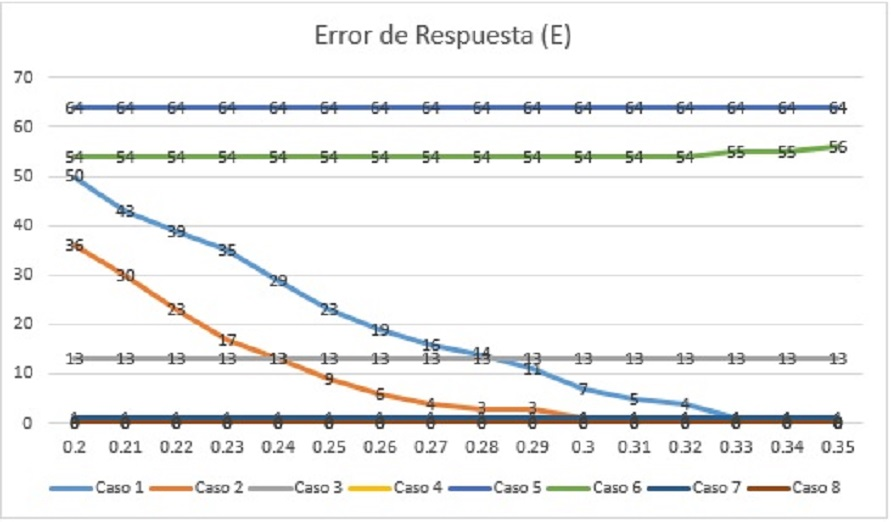
\includegraphics[width=0.7\textwidth]{Imagenes/Cap4/image001}
\end{center}
\begin{center}
\vskip -0.5cm
\caption{\small{Número de errores en la respuesta del sistema para U2.}}
\label{fig:figura4.1}
{\small{Fuente: Elaboración propia}}
\end{center}
\end{figure}


\begin{figure}[H]
\begin{center}
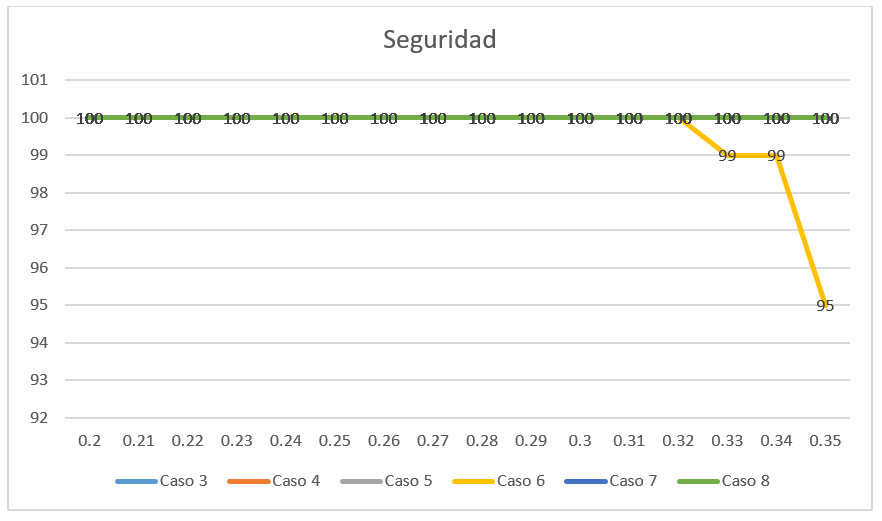
\includegraphics[width=0.7\textwidth]{Imagenes/Cap4/image002}
\end{center}
\begin{center}
\vskip -0.5cm
\caption{\small{Seguridad del sistema para U2.}}
\label{fig:figura4.2}
{\small{Fuente: Elaboración propia}}
\end{center}
\end{figure}

\subsection{Prueba para obtener U1}
\par
En esta segunda prueba se obtuvo que el mejor valor para $U1$ es 0.51. Esto porque, se observó que para los casos 1, 2 y 7, ver Tablas \ref{table:tabla4.9} y \ref{table:tabla4.10}, cualquier valor que tome $U1$ entre 0.40 y 0.55 el valor de $E$ es el mismo, por lo que no se tomó en cuenta a estos casos, entonces para los casos 3, 4 y 8 se observó que conforme $U1$ aumenta de valor $E$ también aumenta, por otro lado, para los casos 5 y 6 si $U1$ aumenta $E$ disminuye, por ello se escogió a 0.51 como valor intermedio para los casos 3, 4, 5, 6 y 8, ver la Figura \ref{fig:figura4.3}. Además, el sistema no dejo pasar en ningún caso a intrusos por lo que se alcanzó un 100\% en seguridad, ver la Figura \ref{fig:figura4.4}.

\begin{center}
\begin{table}[H]
\centering
\caption{\small{Resultados para obtener U1 en el caso 1.}}
\label{table:tabla4.9}
\vskip 0.2cm
\scalebox{0.7}{
\begin{tabular}{|c|c|c|c|c|c|c|c|}
\hline 
U1 & U2 & IC & FI & NI & A & D & E \\
\hline 
0.40 & 0.31 & 95 & 5 & 0 & 100 & 0 & 5 \\
\hline 
0.41 & 0.31 & 95 & 5 & 0 & 100 & 0 & 5 \\
\hline 
0.42 & 0.31 & 95 & 5 & 0 & 100 & 0 & 5 \\
\hline 
0.43 & 0.31 & 95 & 5 & 0 & 100 & 0 & 5 \\
\hline 
0.44 & 0.31 & 95 & 5 & 0 & 100 & 0 & 5 \\
\hline 
0.45 & 0.31 & 95 & 5 & 0 & 100 & 0 & 5 \\
\hline 
0.46 & 0.31 & 95 & 5 & 0 & 100 & 0 & 5 \\
\hline 
0.47 & 0.31 & 95 & 5 & 0 & 100 & 0 & 5 \\
\hline 
0.48 & 0.31 & 95 & 5 & 0 & 100 & 0 & 5 \\
\hline 
0.49 & 0.31 & 95 & 5 & 0 & 100 & 0 & 5 \\
\hline 
0.50 & 0.31 & 95 & 5 & 0 & 100 & 0 & 5 \\
\hline 
0.51 & 0.31 & 95 & 5 & 0 & 100 & 0 & 5 \\
\hline 
0.52 & 0.31 & 95 & 5 & 0 & 100 & 0 & 5 \\
\hline 
0.53 & 0.31 & 95 & 5 & 0 & 100 & 0 & 5 \\
\hline 
0.54 & 0.31 & 95 & 5 & 0 & 100 & 0 & 5 \\
\hline 
0.55 & 0.31 & 95 & 5 & 0 & 100 & 0 & 5 \\
\hline 
\end{tabular} 
}
\begin{center}
\vskip 0.2cm
{\small{Fuente: Elaboración propia}}
\end{center}
\end{table}
\end{center}

\vskip -1.0cm

\begin{center}
\begin{table}[H]
\centering
\caption{\small{Resultados para obtener U1 en el caso 2.}}
\label{table:tabla4.10}
\vskip 0.2cm
\scalebox{0.7}{
\begin{tabular}{|c|c|c|c|c|c|c|c|}
\hline 
U1 & U2 & IC & FI & NI & A & D & E \\
\hline 
0.40 & 0.31 & 99 & 1 & 0 & 100 & 0 & 1 \\
\hline 
0.41 & 0.31 & 99 & 1 & 0 & 100 & 0 & 1 \\
\hline 
0.42 & 0.31 & 99 & 1 & 0 & 100 & 0 & 1 \\
\hline 
0.43 & 0.31 & 99 & 1 & 0 & 100 & 0 & 1 \\
\hline 
0.44 & 0.31 & 99 & 1 & 0 & 100 & 0 & 1 \\
\hline 
0.45 & 0.31 & 99 & 1 & 0 & 100 & 0 & 1 \\
\hline 
0.46 & 0.31 & 99 & 1 & 0 & 100 & 0 & 1 \\
\hline 
0.47 & 0.31 & 99 & 1 & 0 & 100 & 0 & 1 \\
\hline 
0.48 & 0.31 & 99 & 1 & 0 & 100 & 0 & 1 \\
\hline 
0.49 & 0.31 & 99 & 1 & 0 & 100 & 0 & 1 \\
\hline 
0.50 & 0.31 & 99 & 1 & 0 & 100 & 0 & 1 \\
\hline 
0.51 & 0.31 & 99 & 1 & 0 & 100 & 0 & 1 \\
\hline 
0.52 & 0.31 & 99 & 1 & 0 & 100 & 0 & 1 \\
\hline 
0.53 & 0.31 & 99 & 1 & 0 & 100 & 0 & 1 \\
\hline 
0.54 & 0.31 & 99 & 1 & 0 & 100 & 0 & 1 \\
\hline 
0.55 & 0.31 & 99 & 1 & 0 & 100 & 0 & 1 \\
\hline 
\end{tabular} 
}
\begin{center}
\vskip 0.2cm
{\small{Fuente: Elaboración propia}}
\end{center}
\end{table}
\end{center}

\vskip -1.0cm

\begin{center}
\begin{table}[H]
\centering
\caption{\small{Resultados para obtener U1 en el caso 5.}}
\label{table:tabla4.13}
\vskip 0.2cm
\scalebox{0.7}{
\begin{tabular}{|c|c|c|c|c|c|c|c|}
\hline 
U1 & U2 & IC & FI & NI & A & D & E \\
\hline 
0.40 & 0.31 & 0 & 0 & 100 & 90 & 10 & 100 \\
\hline 
0.41 & 0.31 & 0 & 1 & 99 & 90 & 10 & 99 \\
\hline 
0.42 & 0.31 & 0 & 1 & 99 & 90 & 10 & 99 \\
\hline 
0.43 & 0.31 & 0 & 2 & 98 & 90 & 10 & 98 \\
\hline 
0.44 & 0.31 & 0 & 4 & 96 & 90 & 10 & 96 \\
\hline 
0.45 & 0.31 & 0 & 6 & 94 & 90 & 10 & 94 \\
\hline 
0.46 & 0.31 & 0 & 8 & 92 & 90 & 10 & 92 \\
\hline 
0.47 & 0.31 & 0 & 13 & 87 & 90 & 10 & 87 \\
\hline 
0.48 & 0.31 & 0 & 17 & 83 & 90 & 10 & 83 \\
\hline 
0.49 & 0.31 & 0 & 21 & 79 & 90 & 10 & 79 \\
\hline 
0.50 & 0.31 & 0 & 22 & 78 & 90 & 10 & 78 \\
\hline 
0.51 & 0.31 & 0 & 28 & 72 & 90 & 10 & 72 \\
\hline 
0.52 & 0.31 & 0 & 32 & 68 & 90 & 10 & 68 \\
\hline 
0.53 & 0.31 & 0 & 40 & 60 & 90 & 10 & 60 \\
\hline 
0.54 & 0.31 & 0 & 46 & 54 & 90 & 10 & 54 \\
\hline 
0.55 & 0.31 & 0 & 51 & 49 & 90 & 10 & 51 \\
\hline 
\end{tabular} 
}
\begin{center}
\vskip 0.2cm
{\small{Fuente: Elaboración propia}}
\end{center}
\end{table}
\end{center}

\vskip -1.0cm

\begin{center}
\begin{table}[H]
\centering
\caption{\small{Resultados para obtener U1 en el caso 6.}}
\label{table:tabla4.14}
\vskip 0.2cm
\scalebox{0.7}{
\begin{tabular}{|c|c|c|c|c|c|c|c|}
\hline 
U1 & U2 & IC & FI & NI & A & D & E \\
\hline 
0.40 & 0.31 & 0 & 28 & 72 & 100 & 0 & 72 \\
\hline 
0.41 & 0.31 & 0 & 37 & 63 & 100 & 0 & 63 \\
\hline 
0.42 & 0.31 & 0 & 42 & 58 & 100 & 0 & 58 \\
\hline 
0.43 & 0.31 & 0 & 57 & 43 & 100 & 0 & 43 \\
\hline 
0.44 & 0.31 & 0 & 67 & 33 & 100 & 0 & 33 \\
\hline 
0.45 & 0.31 & 0 & 71 & 29 & 100 & 0 & 29 \\
\hline 
0.46 & 0.31 & 0 & 78 & 22 & 100 & 0 & 22 \\
\hline 
0.47 & 0.31 & 0 & 84 & 16 & 100 & 0 & 16 \\
\hline 
0.48 & 0.31 & 0 & 87 & 13 & 100 & 0 & 13 \\
\hline 
0.49 & 0.31 & 0 & 92 & 8 & 100 & 0 & 8 \\
\hline 
0.50 & 0.31 & 0 & 96 & 4 & 100 & 0 & 4 \\
\hline  
0.51 & 0.31 & 0 & 98 & 2 & 100 & 0 & 2 \\
\hline 
0.52 & 0.31 & 0 & 98 & 2 & 100 & 0 & 2 \\
\hline 
0.53 & 0.31 & 0 & 99 & 1 & 100 & 0 & 1 \\
\hline 
0.54 & 0.31 & 0 & 100 & 0 & 100 & 0 & 0 \\
\hline 
0.55 & 0.31 & 0 & 100 & 0 & 100 & 0 & 0 \\
\hline 
\end{tabular} 
}
\begin{center}
\vskip 0.2cm
{\small{Fuente: Elaboración propia}}
\end{center}
\end{table}
\end{center}


\begin{figure}[H]
\begin{center}
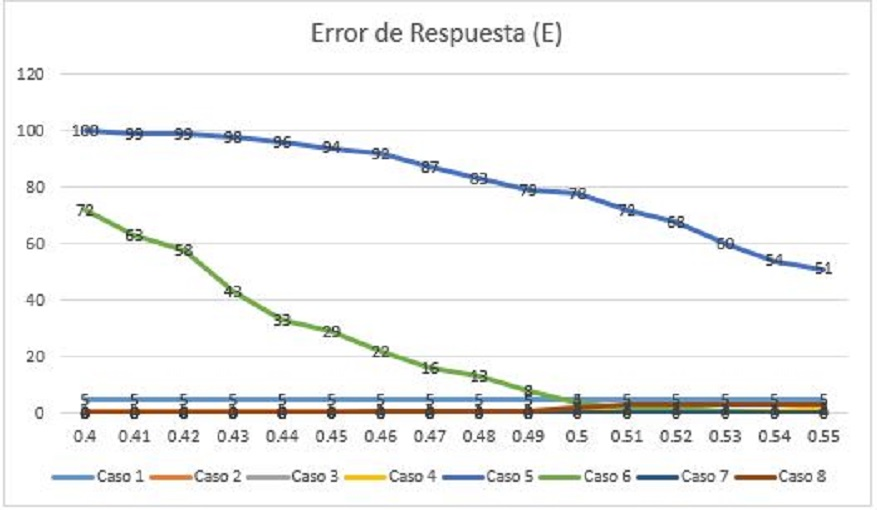
\includegraphics[width=0.7\textwidth]{Imagenes/Cap4/image003}
\end{center}
\begin{center}
\vskip -0.5cm
\caption{\small{Número de errores en la respuesta del sistema para U1.}}
\label{fig:figura4.3}
{\small{Fuente: Elaboración propia}}
\end{center}
\end{figure}

\begin{figure}[H]
\begin{center}
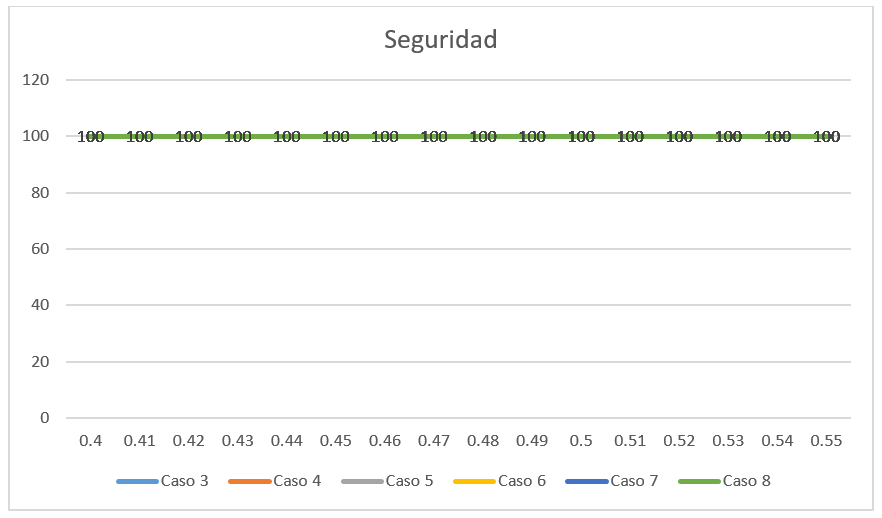
\includegraphics[width=0.7\textwidth]{Imagenes/Cap4/image004}
\end{center}
\begin{center}
\vskip -0.5cm
\caption{\small{Seguridad del sistema para U1.}}
\label{fig:figura4.4}
{\small{Fuente: Elaboración propia}}
\end{center}
\end{figure}

De esta primera etapa se puede concluir que los valores para los umbrales $U1$ y $U2$ son, para $U2 = 0.31$ sin embargo todavía no hemos evaluado cual es el mejor valor para $U1$ si $U$ o 0.51, para ello haremos una comparación del total de errores obtenidos para esto dos valores.

\begin{center}
\begin{table}[H]
\centering
\caption{\small{Comparación de numero de errores entre U1 = U y U1 = 0.51.}}
\label{table:tabla4.17}
\vskip 0.2cm
\scalebox{0.7}{
\begin{tabular}{|c|c|c|c|}
\hline 
$N^\circ$ & U2 & U1=U & U1=0.51 \\
\hline 
1 & 0.31 & 5 & 5 \\
\hline 
2 & 0.31 & 1 & 1 \\
\hline 
3 & 0.31 & 13 & 0 \\
\hline 
4 & 0.31 & 0 & 1 \\
\hline 
5 & 0.31 & 64 & 72 \\
\hline 
6 & 0.31 & 54 & 2 \\
\hline 
7 & 0.31 & 1 & 0 \\
\hline 
8 & 0.31 & 0 & 3 \\
\hline 
\multicolumn{2}{|c|}{Total de Error} & 138 & 84 \\
\hline
\end{tabular} 
}
\begin{center}
\vskip 0.2cm
{\small{Fuente: Elaboración propia}}
\end{center}
\end{table}
\end{center}

Podemos ver en la Tabla \ref{table:tabla4.17} que para $U1 = 0.51$ se obtuvo una menor cantidad de número de errores en la respuesta del sistema de reconocimiento de voz, debido a esto se escogerá este valor.
\vskip 0.5cm
Ahora evaluaremos el tiempo de ejecución que toma el sistema para realizar el reconocimiento de voz y el reajuste de los umbrales, si bien este último no es necesario evaluar ya que el valor de $U1$ es 0.51 un valor estático y no dinámico (calculado por la Ecuación \eqref{eq:ecuacion105}), de todas maneras se realizará como información complementaria para la investigación.

\newpage
\begin{figure}[H]
\captionsetup{justification=centering}
\begin{center}
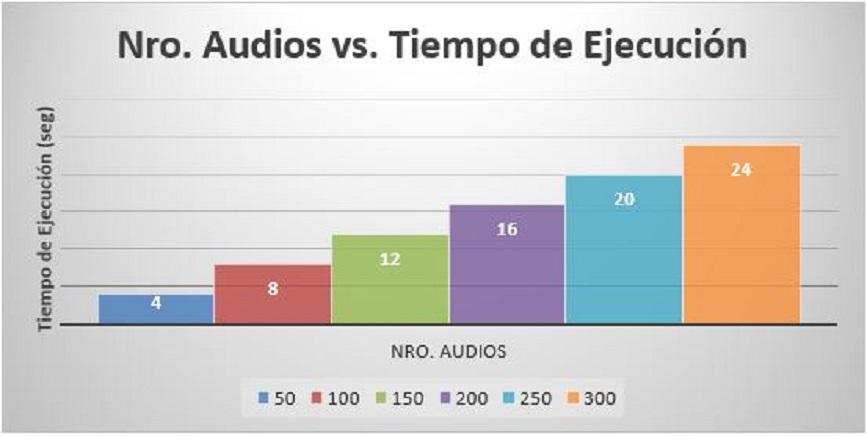
\includegraphics[width=0.6\textwidth]{Imagenes/Cap4/image005}
\end{center}
\begin{center}
\vskip -0.5cm
\caption{\small{Gráfico de barras del tiempo de ejecución para el reconocimiento de voz.}}
\label{fig:figura4.5}
{\small{Fuente: Elaboración propia}}
\end{center}
\end{figure}
\vskip -0.5cm
\begin{figure}[H]
\captionsetup{justification=centering}
\begin{center}
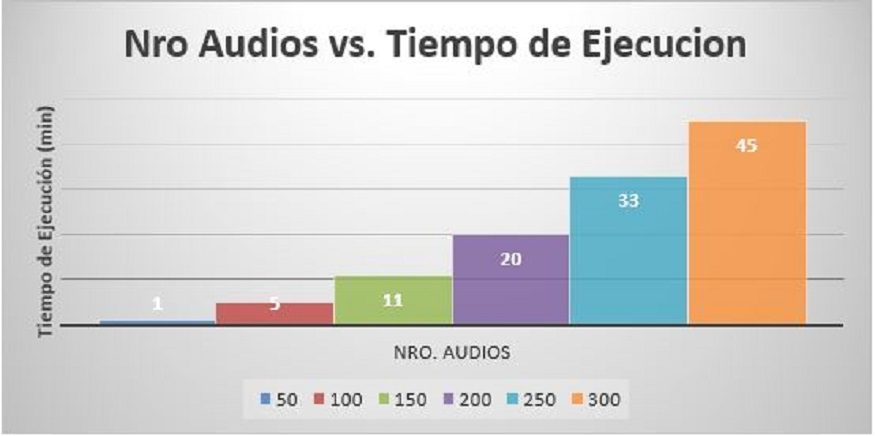
\includegraphics[width=0.6\textwidth]{Imagenes/Cap4/image006}
\end{center}
\begin{center}
\vskip -0.5cm
\caption{\small{Gráfico de barras del tiempo de ejecución para el reajuste del umbral U1.}}
\label{fig:figura4.6}
{\small{Fuente: Elaboración propia}}
\end{center}
\end{figure}
\vskip -0.5cm
Como podemos ver en la Figura \ref{fig:figura4.5} el gráfico muestra una pendiente de función lineal, conforme aumentamos el número de audios en la base de datos el tiempo de ejecución para la respuesta del sistema aumenta, por lo que esta puede ser calculada por la siguiente fórmula:

\begin{equation}
\label{eq:ecuacion4.1}
TE = t x N
\end{equation}

Donde:
\begin{enumerate}
\item[-]\textit{TE}: Tiempo de ejecución para la respuesta del sistema
\item[-]\textit{t}: Tiempo que demora en comparar dos audios
\item[-]\textit{N}: Número total de audios en la base de datos
\end{enumerate}

\vskip 0.5cm
De la Ecuación \eqref{eq:ecuacion4.1} y los datos obtenidos que se ve en la Figura \ref{fig:figura4.5}, se tiene que el valor de $t$ es 0.08 segundos, este valor varía de acuerdo al hardware del dispositivo en donde se implemente el sistema, para nuestro proyecto hemos usado un dispositivo móvil Android Samsung J6+ con un procesador de 4 núcleos de 1.8 GHz.
\vskip 0.5cm
El tiempo de respuesta del sistema para el reconocimiento de voz no debe ser mayor a 5 segundos tal como se definió en las características generales del ciclo de negocio de la arquitectura del sistema en la Tabla \ref{table:tabla3.1}, sin embargo, si se utiliza un número mayor a 60 audios (patrones característicos) en la base de datos, entonces no se cumplirá con este requisito que se planteó.
\vskip 0.5cm
Por ello, se planteó utilizar la técnica para la construcción del patrón de referencia definida por la Ecuación \eqref{eq:ecuacion101} que consiste en agrupar un número de audios y dar como resultado un patrón promedio que los represente, así podremos disminuir el tiempo de respuesta del sistema al tener un número menor de patrones en la base de datos.

\section{Pruebas para la construcción del patrón de referencia}
En esta segunda parte al igual que la primera consta de 2 etapas, en la primera el umbral $U1$ se considerará con valor dinámico es decir el valor definido por la Ecuación \eqref{eq:ecuacion105} y para la segunda etapa el umbral $U1$ tendrá un valor estático que será 0.51. De esta manera procederemos a evaluar el algoritmo de construcción del patrón de referencia en estos dos escenarios.
\vskip 0.5cm
A continuación, veremos los resultados que se obtuvieron en la realización de las pruebas para los 8 escenarios o casos definidos anteriormente, donde $N$ representa el número de patrones o audios que se emplearán para la construcción del patrón de referencia.

\subsection{Prueba con U1 dinámico}
\par
De esta primera prueba se obtuvo que el mejor valor para $N$ es 5. Esto porque, se observó que para los casos 3, 4, 7 y 8 cualquier valor que tome $N$ el valor de $E = 0$, por lo que no se tomó en cuenta a estos casos, entonces para los casos 1, 2, 5 y 6, ver Tablas \ref{table:tabla4.18}, \ref{table:tabla4.19}, \ref{table:tabla4.22}, \ref{table:tabla4.23}, se observó que el mejor valor para $N$ es 5, ver la Figura \ref{fig:figura4.7}, si bien los valores de $E$ son grandes, por otro lado, $IC = 0$ por lo que en ningún caso se dejo pasar a intrusos, por lo tanto, se obtuvo un 100\% en seguridad del sistema, ver la Figura \ref{fig:figura4.8}.

\begin{center}
\begin{table}[H]
\centering
\caption{\small{Resultados para el caso 1 con U1 dinámico.}}
\label{table:tabla4.18}
\scalebox{0.7}{
\begin{tabular}{|c|c|c|c|c|c|c|c|c|}
\hline 
$N^\circ$ & U1 & U2 & IC & FI & NI & A & D & E \\
\hline 
5 & U & 0.31 & 85 & 7 & 8 & 100 & 0 & 15 \\
\hline 
6 & U & 0.31 & 75 & 9 & 16 & 100 & 0 & 25 \\
\hline 
7 & U & 0.31 & 69 & 4 & 27 & 100 & 0 & 31 \\
\hline 
8 & U & 0.31 & 57 & 0 & 43 & 100 & 0 & 43 \\
\hline 
9 & U & 0.31 & 55 & 4 & 41 & 100 & 0 & 45 \\
\hline 
10 & U & 0.31 & 68 & 8 & 24 & 100 & 0 & 32 \\
\hline 
\end{tabular} 
}
\begin{center}
\vskip 0.2cm
{\small{Fuente: Elaboración propia}}
\end{center}
\end{table}
\end{center}

\begin{center}
\begin{table}[H]
\centering
\caption{\small{Resultados para el caso 2 con U1 dinámico.}}
\label{table:tabla4.19}
\scalebox{0.7}{
\begin{tabular}{|c|c|c|c|c|c|c|c|c|}
\hline 
$N^\circ$ & U1 & U2 & IC & FI & NI & A & D & E \\
\hline 
5 & U & 0.31 & 86 & 0 & 14 & 100 & 0 & 14 \\
\hline 
6 & U & 0.31 & 87 & 0 & 13 & 100 & 0 & 13 \\
\hline 
7 & U & 0.31 & 76 & 1 & 23 & 100 & 0 & 24 \\
\hline 
8 & U & 0.31 & 60 & 0 & 40 & 100 & 0 & 40 \\
\hline 
9 & U & 0.31 & 71 & 0 & 29 & 100 & 0 & 29 \\
\hline 
10 & U & 0.31 & 78 & 0 & 22 & 100 & 0 & 22 \\
\hline 
\end{tabular} 
}
\begin{center}
\vskip 0.2cm
{\small{Fuente: Elaboración propia}}
\end{center}
\end{table}
\end{center}

\begin{center}
\begin{table}[H]
\centering
\caption{\small{Resultados para el caso 5 con U1 dinámico.}}
\label{table:tabla4.22}
\scalebox{0.7}{
\begin{tabular}{|c|c|c|c|c|c|c|c|c|}
\hline 
$N^\circ$ & U1 & U2 & IC & FI & NI & A & D & E \\
\hline 
5 & U & 0.31 & 0 & 3 & 97 & 86 & 14 & 97 \\
\hline 
6 & U & 0.31 & 0 & 4 & 96 & 88 & 12 & 96 \\
\hline 
7 & U & 0.31 & 0 & 2 & 98 & 92 & 8 & 98 \\
\hline 
8 & U & 0.31 & 0 & 0 & 100 & 93 & 7 & 100 \\
\hline 
9 & U & 0.31 & 0 & 0 & 100 & 83 & 17 & 100 \\
\hline 
10 & U & 0.31 & 0 & 5 & 95 & 83 & 17 & 95 \\
\hline 
\end{tabular} 
}
\begin{center}
\vskip 0.2cm
{\small{Fuente: Elaboración propia}}
\end{center}
\end{table}
\end{center}


\begin{center}
\begin{table}[H]
\centering
\caption{\small{Resultados para el caso 6 con U1 dinámico.}}
\label{table:tabla4.23}
\scalebox{0.7}{
\begin{tabular}{|c|c|c|c|c|c|c|c|c|}
\hline 
$N^\circ$ & U1 & U2 & IC & FI & NI & A & D & E \\
\hline 
5 & U & 0.31 & 0 & 0 & 100 & 100 & 0 & 100 \\
\hline 
6 & U & 0.31 & 0 & 0 & 100 & 100 & 0 & 100 \\
\hline 
7 & U & 0.31 & 0 & 1 & 99 & 100 & 0 & 99 \\
\hline 
8 & U & 0.31 & 0 & 0 & 100 & 100 & 0 & 100 \\
\hline 
9 & U & 0.31 & 0 & 4 & 96 & 100 & 0 & 96 \\
\hline 
10 & U & 0.31 & 0 & 0 & 100 & 100 & 0 & 100 \\
\hline 
\end{tabular} 
}
\begin{center}
\vskip 0.2cm
{\small{Fuente: Elaboración propia}}
\end{center}
\end{table}
\end{center}

\begin{figure}[H]
\begin{center}
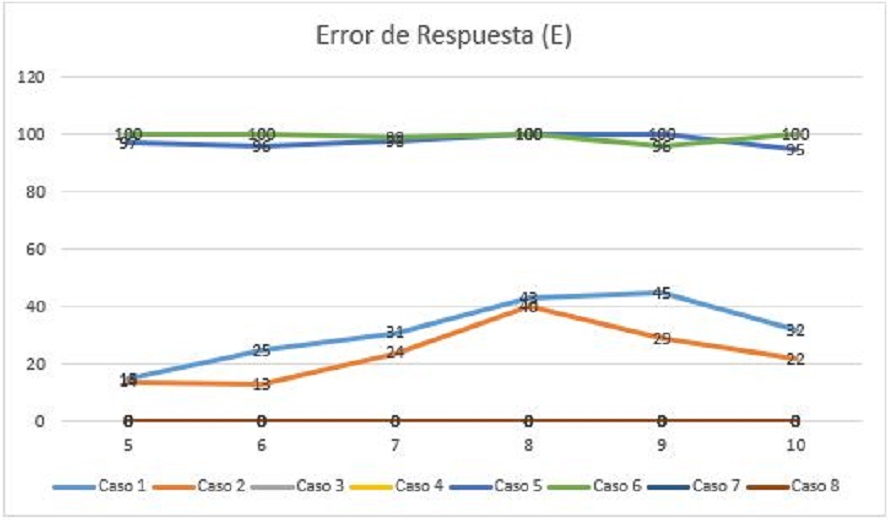
\includegraphics[width=0.7\textwidth]{Imagenes/Cap4/image007}
\end{center}
\begin{center}
\vskip -0.5cm
\caption{\small{Número de errores en la respuesta del sistema para U1 dinámico.}}
\label{fig:figura4.7}
{\small{Fuente: Elaboración propia}}
\end{center}
\end{figure}

\vskip -0.5cm

\begin{figure}[H]
\begin{center}
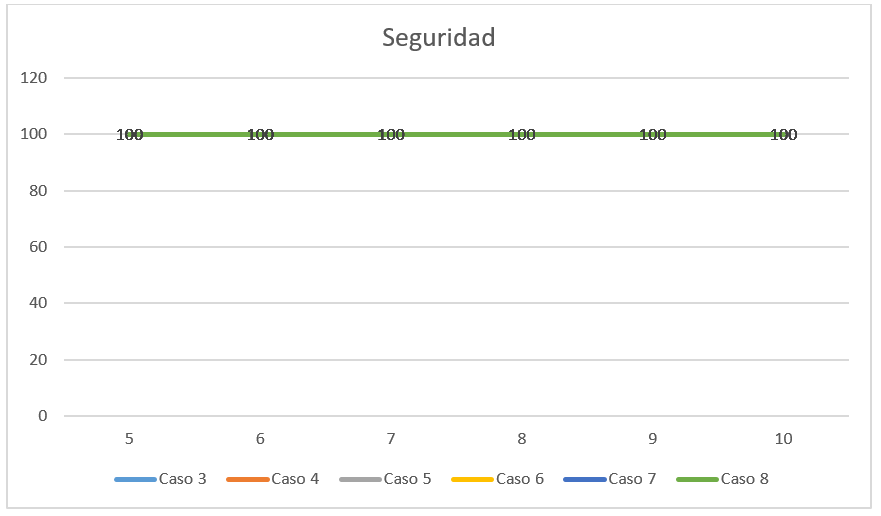
\includegraphics[width=0.7\textwidth]{Imagenes/Cap4/image008}
\end{center}
\begin{center}
\vskip -0.5cm
\caption{\small{Seguridad del sistema para U1 dinámico.}}
\label{fig:figura4.8}
{\small{Fuente: Elaboración propia}}
\end{center}
\end{figure}

\subsection{Prueba con U1 estático}
\par
De esta segunda prueba se obtuvo que el mejor valor para $N$ es 5. Esto porque, se observó que para los casos 3, 4 y 7 cualquier valor que tome $N$ el valor de $E = 0$, por lo que no se tomó en cuenta a estos casos, entonces para los casos 1, 2, 5, 6 y 8, ver Tablas \ref{table:tabla4.26}, \ref{table:tabla4.27}, \ref{table:tabla4.30} y \ref{table:tabla4.31}, podemos ver que el mejor valor para $N$ es 5, ver la Figura \ref{fig:figura4.9}, si bien los valores de $E$ son grandes, por otro lado, $IC = 0$ por lo que en ningún caso se dejo pasar a intrusos, por lo tanto, se obtuvo un 100\% en seguridad del sistema, ver la Figura \ref{fig:figura4.10}.

\begin{center}
\begin{table}[H]
\centering
\caption{\small{Resultados para el caso 1 con U1 estático.}}
\label{table:tabla4.26}
\scalebox{0.7}{
\begin{tabular}{|c|c|c|c|c|c|c|c|c|}
\hline 
$N^\circ$ & U1 & U2 & IC & FI & NI & A & D & E \\
\hline 
5 & 0.51 & 0.31 & 92 & 8 & 0 & 100 & 0 & 8 \\
\hline 
6 & 0.51 & 0.31 & 89 & 11 & 0 & 100 & 0 & 11 \\
\hline 
7 & 0.51 & 0.31 & 90 & 10 & 0 & 100 & 0 & 10 \\
\hline 
8 & 0.51 & 0.31 & 81 & 19 & 0 & 100 & 0 & 19 \\
\hline 
9 & 0.51 & 0.31 & 83 & 17 & 0 & 100 & 0 & 17 \\
\hline 
10 & 0.51 & 0.31 & 91 & 10 & 0 & 100 & 0 & 10 \\
\hline 
\end{tabular} 
}
\begin{center}
\vskip 0.2cm
{\small{Fuente: Elaboración propia}}
\end{center}
\end{table}
\end{center}

\begin{center}
\begin{table}[H]
\centering
\caption{\small{Resultados para el caso 2 con U1 estático.}}
\label{table:tabla4.27}
\scalebox{0.7}{
\begin{tabular}{|c|c|c|c|c|c|c|c|c|}
\hline 
$N^\circ$ & U1 & U2 & IC & FI & NI & A & D & E \\
\hline 
5 & 0.51 & 0.31 & 99 & 1 & 0 & 100 & 0 & 1 \\
\hline 
6 & 0.51 & 0.31 & 99 & 1 & 0 & 100 & 0 & 1 \\
\hline 
7 & 0.51 & 0.31 & 98 & 2 & 0 & 100 & 0 & 2 \\
\hline 
8 & 0.51 & 0.31 & 99 & 1 & 0 & 100 & 0 & 1 \\
\hline 
9 & 0.51 & 0.31 & 98 & 2 & 0 & 100 & 0 & 2 \\
\hline 
10 & 0.51 & 0.31 & 99 & 1 & 0 & 100 & 0 & 1 \\
\hline 
\end{tabular} 
}
\begin{center}
\vskip 0.2cm
{\small{Fuente: Elaboración propia}}
\end{center}
\end{table}
\end{center}

\begin{center}
\begin{table}[H]
\centering
\caption{\small{Resultados para el caso 5 con U1 estático.}}
\label{table:tabla4.30}
\scalebox{0.7}{
\begin{tabular}{|c|c|c|c|c|c|c|c|c|}
\hline 
$N^\circ$ & U1 & U2 & IC & FI & NI & A & D & E \\
\hline 
5 & 0.51 & 0.31 & 0 & 17 & 83 & 86 & 14 & 83 \\
\hline 
6 & 0.51 & 0.31 & 0 & 20 & 80 & 88 & 12 & 80 \\
\hline 
7 & 0.51 & 0.31 & 0 & 19 & 81 & 92 & 8 & 81 \\
\hline 
8 & 0.51 & 0.31 & 0 & 5 & 95 & 93 & 7 & 95 \\
\hline 
9 & 0.51 & 0.31 & 0 & 8 & 92 & 83 & 17 & 92 \\
\hline 
10 & 0.51 & 0.31 & 0 & 16 & 84 & 83 & 17 & 84 \\
\hline 
\end{tabular} 
}
\begin{center}
\vskip 0.2cm
{\small{Fuente: Elaboración propia}}
\end{center}
\end{table}
\end{center}


\begin{center}
\begin{table}[H]
\centering
\caption{\small{Resultados para el caso 6 con U1 estático.}}
\label{table:tabla4.31}
\scalebox{0.7}{
\begin{tabular}{|c|c|c|c|c|c|c|c|c|}
\hline 
$N^\circ$ & U1 & U2 & IC & FI & NI & A & D & E \\
\hline 
5 & 0.51 & 0.31 & 0 & 94 & 6 & 100 & 0 & 6 \\
\hline 
6 & 0.51 & 0.31 & 0 & 76 & 24 & 100 & 0 & 24 \\
\hline 
7 & 0.51 & 0.31 & 0 & 82 & 18 & 100 & 0 & 18 \\
\hline 
8 & 0.51 & 0.31 & 0 & 56 & 44 & 100 & 0 & 44 \\
\hline 
9 & 0.51 & 0.31 & 0 & 61 & 39 & 100 & 0 & 39 \\
\hline 
10 & 0.51 & 0.31 & 0 & 65 & 35 & 100 & 0 & 35 \\
\hline 
\end{tabular} 
}
\begin{center}
\vskip 0.2cm
{\small{Fuente: Elaboración propia}}
\end{center}
\end{table}
\end{center}


\begin{figure}[H]
\begin{center}
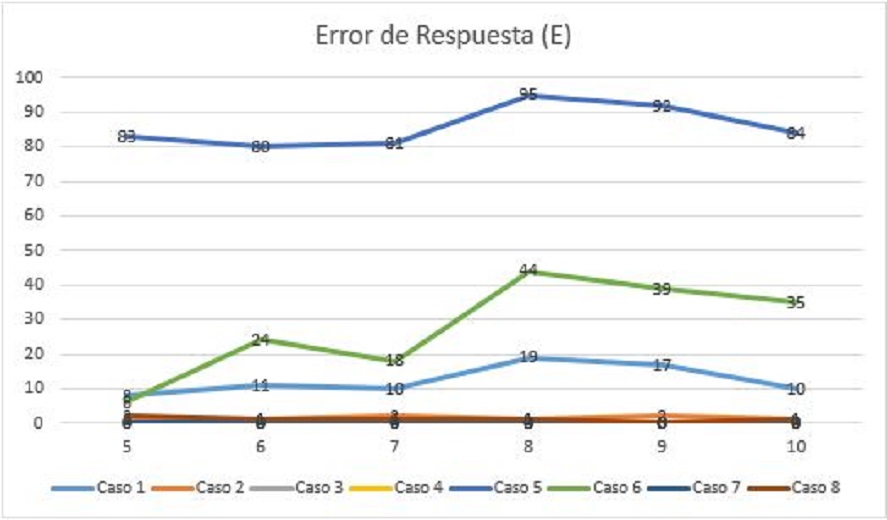
\includegraphics[width=0.7\textwidth]{Imagenes/Cap4/image009}
\end{center}
\begin{center}
\vskip -0.5cm
\caption{\small{Número de errores en la respuesta del sistema para U1 estático.}}
\label{fig:figura4.9}
{\small{Fuente: Elaboración propia}}
\end{center}
\end{figure}

\vskip -0.5cm

\begin{figure}[H]
\begin{center}
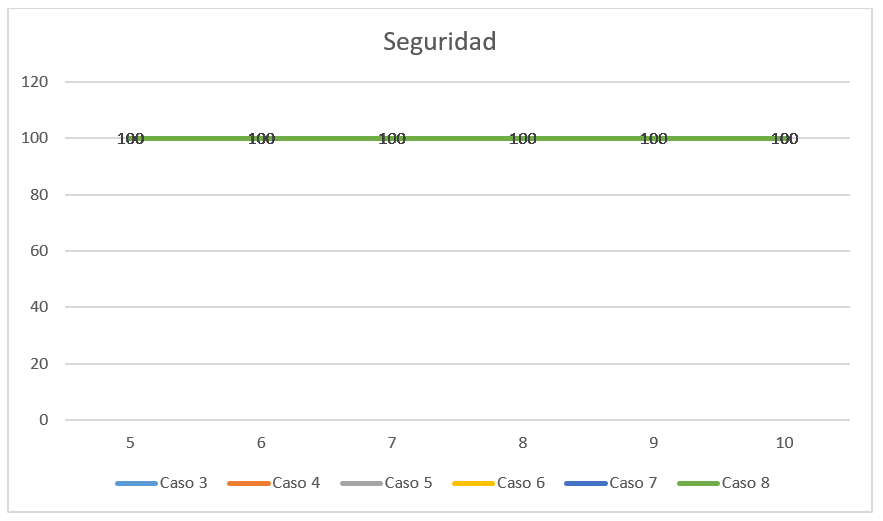
\includegraphics[width=0.7\textwidth]{Imagenes/Cap4/image010}
\end{center}
\begin{center}
\vskip -0.5cm
\caption{\small{Seguridad del sistema para U1 estático.}}
\label{fig:figura4.10}
{\small{Fuente: Elaboración propia}}
\end{center}
\end{figure}

Después de realizar todas las pruebas para poder hallar el mejor valor para $N$ (número de patrones para la construcción del patrón de referencia) podemos ver que se obtuvieron mejores resultados para $N = 5$, además que sigue siendo el mejor valor para $U1 = 0.51$ y no el valor definido por la Ecuación \eqref{eq:ecuacion101}, por lo que queda totalmente corroborado que este es el mejor valor. 
\vskip 0.5cm
Si bien con $N = 5$ disminuimos en la quinta parte el tiempo de ejecución en la respuesta para el reconocimiento del locutor en el sistema, todavía no hemos comparado si este tiene menos errores que $N = 1$, a continuación, en la Tabla \ref{table:tabla4.34} veremos la cantidad de errores que se obtuvieron para estos dos casos.

\begin{center}
\begin{table}[H]
\centering
\caption{\small{Comparación de numero de errores entre U1 = U y U1 = 0.51.}}
\label{table:tabla4.34}
\vskip 0.2cm
\scalebox{0.7}{
\begin{tabular}{|c|c|c|c|c|}
\hline 
$N^\circ$ & U1 & U2 & N=1 & N=5 \\
\hline 
1 & 0.51 & 0.31 & 5 & 8 \\
\hline 
2 & 0.51 & 0.31 & 1 & 1 \\
\hline 
3 & 0.51 & 0.31 & 0 & 0 \\
\hline 
4 & 0.51 & 0.31 & 1 & 0 \\
\hline 
5 & 0.51 & 0.31 & 72 & 83 \\
\hline 
6 & 0.51 & 0.31 & 2 & 6 \\
\hline 
7 & 0.51 & 0.31 & 0 & 0 \\
\hline 
8 & 0.51 & 0.31 & 3 & 2 \\
\hline 
\multicolumn{3}{|c|}{Total de Error} & 84 & 100 \\
\hline
\end{tabular} 
}
\begin{center}
\vskip 0.2cm
{\small{Fuente: Elaboración propia}}
\end{center}
\end{table}
\end{center}

De la Tabla \ref{table:tabla4.34} podemos ver que para $N = 1$ se tiene un \textit{total de error} de 84 de un total de 800 pruebas haciendo una tasa de error del 10.5\%, mientras que para $N = 5$ se tiene un \textit{total de error} de 100 haciendo una tasa de error del 12.5\%, por lo que se escogerá a $N = 1$, es decir que no se aplicará el algoritmo de construcción de patrón de referencia definido por la Ecuación \eqref{eq:ecuacion101}. 
\vskip 0.5cm
Si bien con $N = 5$ disminuiríamos el tiempo de respuesta del reconocimiento del locutor del sistema, este presenta un problema para el caso 1 debido a que se tiene $E = 8$ resultando una tasa de error del 92\% en la respuesta del sistema incumpliendo con los requisitos definidos para la arquitectura del sistema en el ciclo de negocio, el cual se estableció como mínimo un 95\% en la tasa de acierto, requisito que si cumple para $N = 1$.

\subsection{Prueba de hipótesis o de significación}
Como se dijo anteriormente para efectuar el análisis estadístico de los datos se hará la prueba de independencia Chi- Cuadrado de Pearson para dos variables nominales, ver en Apéndice A.

\begin{enumerate}
\item[1.] La Tabla \ref{table:tabla4.35} muestra los resultados obtenidos del experimento con $U1 = 0.51$ y $U2 = 0.31$, estos datos son las frecuencias observadas (FO), elaborando así la tabla de contingencia.

\begin{center}
\begin{table}[H]
\centering
\caption{\small{Tabla de contingencia o de frecuencias observadas.}}
\label{table:tabla4.35}
\vskip 0.2cm
\scalebox{0.7}{
\begin{tabular}{|c|c|c|c|c|c|}
\hline 
CA/RV & IC & FI & NI & TOTAL \\
\hline 
C1 & 95 & 5 & 0 & 100 \\
\hline 
C2 & 99 & 1 & 0 & 100 \\
\hline 
C3 & 0 & 0 & 100 & 100 \\
\hline 
C4 & 0 & 1 & 99 & 100 \\
\hline 
C5 & 0 & 28 & 72 & 100 \\
\hline 
C6 & 0 & 98 & 2 & 100 \\
\hline 
C7 & 0 & 0 & 100 & 100 \\
\hline 
C8 & 0 & 3 & 97 & 100 \\
\hline 
TOTAL & 194 & 136 & 470 & 800 \\
\hline
\end{tabular} 
}
\begin{center}
\vskip 0.2cm
{\small{Fuente: Elaboración propia}}
\end{center}
\end{table}
\end{center}

\item[2.] La Tabla \ref{table:tabla4.36} muestra el cálculo de la frecuencia esperada (FE).

\begin{center}
\begin{table}[H]
\centering
\caption{\small{Tabla de frecuencias esperadas.}}
\label{table:tabla4.36}
\vskip 0.2cm
\scalebox{0.7}{
\begin{tabular}{|c|c|c|c|c|c|}
\hline 
CA/RV & IC & FI & NI & TOTAL \\
\hline 
C1 & 24.25 & 17 & 58.75 & 100 \\
\hline 
C2 & 24.25 & 17 & 58.75 & 100 \\
\hline 
C3 & 24.25 & 17 & 58.75 & 100 \\
\hline 
C4 & 24.25 & 17 & 58.75 & 100 \\
\hline 
C5 & 24.25 & 17 & 58.75 & 100 \\
\hline 
C6 & 24.25 & 17 & 58.75 & 100 \\
\hline 
C7 & 24.25 & 17 & 58.75 & 100 \\
\hline 
C8 & 24.25 & 17 & 58.75 & 100 \\
\hline 
TOTAL & 194 & 136 & 470 & 800 \\
\hline
\end{tabular} 
}
\begin{center}
\vskip 0.2cm
{\small{Fuente: Elaboración propia}}
\end{center}
\end{table}
\end{center}

\item[3.] Calcular los grados de libertad.
\par
$\alpha = 0.05$ (nivel de confianza del 5\%) \\
$gl = (3-1)(8-1) = 14$ \\
$X^{2}_{cri} = 23.6848$ 

\item[4.]Plantear las hipótesis.
\par
$H_{0}$: La respuesta del reconocimiento de voz utilizando MFCC y DTW es independiente del caso de control de acceso. \\
$H_{1}$: La respuesta del reconocimiento de voz utilizando MFCC y DTW depende del caso de control de acceso.

\item[5.] Construcción de las áreas de aceptación y rechazo.

\begin{figure}[H]
\captionsetup{justification=centering}
\begin{center}
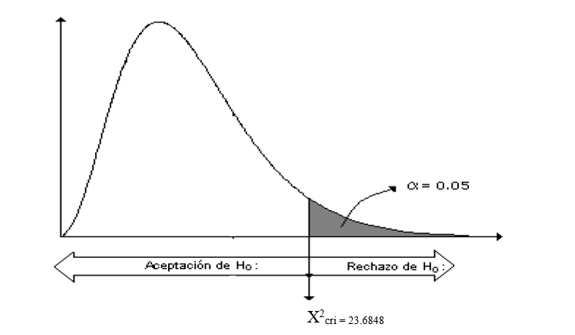
\includegraphics[width=0.6\textwidth]{Imagenes/Cap4/image011}
\end{center}
\begin{center}
\vskip -0.5cm
\caption{\small{ Área de aceptación y rechazo de H0.}}
\label{fig:figura4.11}
{\small{Fuente: Elaboración propia}}
\end{center}
\end{figure}

\newpage
\item[6.]La Tabla \ref{table:tabla4.37} muestra los valores de la diferencia cuadrada de la frecuencia observada con la esperada y luego dividida entre la frecuencia esperada, teniendo todo esto pasaremos a calcular la ji-Cuadrada que no es más que la raíz cuadrada de la sumatoria de estos valores.

\begin{center}
\begin{table}[H]
\centering
\caption{\small{Tabla con los valores ji-cuadrada.}}
\label{table:tabla4.37}
\vskip 0.2cm
\scalebox{0.7}{
\begin{tabular}{|c|c|c|c|c|}
\hline 
CA/RV & IC & FI & NI \\
\hline 
C1 & 206.4149485 & 8.47058824 & 58.75 \\
\hline 
C2 & 230.4149485 & 15.0588235 & 58.75 \\
\hline 
C3 & 24.25 & 17 & 28.962766 \\
\hline 
C4 & 24.25 & 15.0588235 & 27.2755319 \\
\hline 
C5 & 24.25 & 7.11764706 & 2.98829787 \\
\hline 
C6 & 24.25 & 385.941176 & 54.8180851 \\
\hline 
C7 & 24.25 & 17 & 28.962766 \\
\hline 
C8 & 24.25 & 11.5294118 & 24.9031915 \\
\hline
\end{tabular} 
}
\begin{center}
\vskip 0.2cm
{\small{Fuente: Elaboración propia}}
\end{center}
\end{table}
\end{center}

\item[7.] Finalmente se obtuvo un $X^{2}_{exp} = 36.6772$, como podemos ver este valor es mayor al valor de $X^{2}_{cri} = 23.6848$, por lo que la hipótesis nula H0 se rechaza. Entonces podemos decir que con un nivel de confianza del 5\% se encontró que la respuesta del reconocimiento de voz utilizando MFCC y DTW depende del caso de control de acceso. Por lo que se contrasta la hipótesis planteada durante el proceso de elaboración del plan de investigación, es decir, que se logró demostrar la relación entre las variables de estudio formuladas en la investigación, por lo que podemos decir que el acceso a una vivienda puede ser controlado por reconocimiento de voz del locutor dependiente del texto utilizando MFCC Y DTW.

\end{enumerate}







